\section{Tutorial For Simple Strike-Slip Fault}

\subsection{Overview}

In this tutorial we will walk through the steps necessary to
construct, run, and view the results of a benchmark problem involving
a simple, vertical, through-going strike-slip fault. This problem
examines the elastic deformation from a left-lateral earthquake in
3-D without body forces.

\subsection{Problem Description}

The model domain is a cube with edges 1 km long (0 km $\leq$ x $\leq$
1 km; 0 km $\leq$ y $\leq$ 1 km; 0 km $\leq$ z $\leq$ 1 km) and is
composed of two materials. The fault separates two materials that have
the same properties. Both materials are Poisson solids with Lame's
constants ($\mu$ and $\lambda$) equal to 30 GPa.

The strike-slip fault dips at an angle of 90 degrees. The slip
distribution is 1.0 m of uniform left-lateral motion. The face of the
cube on the plane x=0 is held fixed. The other lateral faces and top
and bottom of the mesh are traction-free. The solution to this problem
is zero stresses and strains with no displacements for the region
$x<0.5$ km and a y-displacement of 1.0 m for $x>0.5$ km.

\begin{figure}
  \begin{center}
    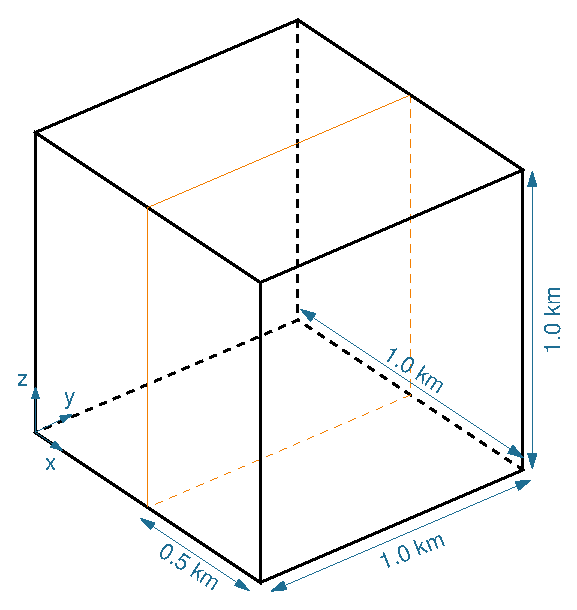
\includegraphics{figs/geometry}
    \caption{Geometry of model domain for simple model with
      strike-slip fault.}
  \end{center}
\end{figure}  

\subsubsection{Workflow}

The complete workflow used to create the input files for this tutorial
is shown in figure~\ref{fig:splitcube:workflow}. 

\begin{figure}[htbp]
  \begin{center}
    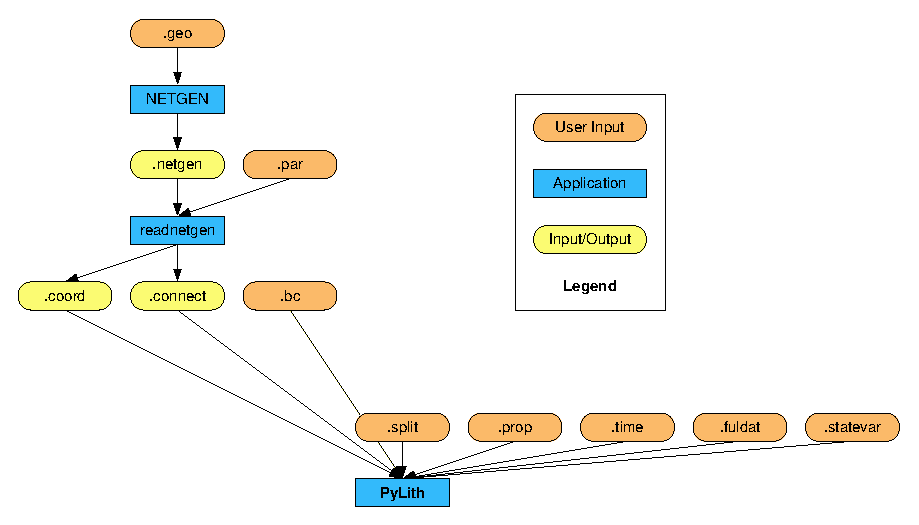
\includegraphics{figs/workflow}
    \caption{Workflow for setting up input files for example with
      simple strike-slip faylt.}
    \label{fig:splitcube:workflow}
  \end{center}
\end{figure}

\subsection{Download and unpack}

We will start by downloading the tutorial tarball and unpacking it.

\begin{enumerate}
\item Download the \href{http://www.geodynamics.org:8080/cig/Members/willic3/pylithusers/pylith0.8/pylith-0.8\_tutorials.tgz}{tutorial tarball}
  and unpack it in a location of your choosing.

  \begin{screen}
    \shellprompt\userinput{tar -zxvf pylith-0.8\_tutorials.tgz}
  \end{screen}
  
\item Go to the \directory{tutorials/splitcube} directory.
  The \directory{archive} directory contains all of the input and
  output files associated with this tutorial. We will copy input files
  from this directory into the \directory{workarea} directory. At each
  step, you can check to make sure your input and output agree with
  the files in the \directory{archive} directory. These files also
  allow you to start at an intermediate step as described in the next
  section.

  \begin{screen}
    \shellprompt\userinput{cd tutorials/splitcube}
  \end{screen}

\end{enumerate}

\subsection{Tutor}

Copy the \filename{tutor.py} script from the \directory{archive}
directory into the \directory{workarea} directory. 

\begin{tip}
  If you have run this tutorial previously, you may want to run
  \command{tutor.py} in mode "clean" with step "all" to clear out all
  old tutorial files.
\end{tip}

\begin{screen}
\shellprompt\userinput{cd workarea}
\shellprompt\userinput{cp ../archive/tutor.py .}
\shellprompt\userinput{./tutor.py -m clean -s all}
\end{screen}

\subsection{Generate the mesh}

In this step we will generate the finite-element mesh for the
benchmark problem using \application{NETGEN}.

\begin{enumerate}
\item In the \directory{splitcube/workarea} directory, run
  \command{tutor.py} for step "mesh" with mode "retrieve" to fetch the
  geometry file for \application{NETGEN}. You may also want to run
  \command{tutor.py} for this step with mode "clean" to clean out old
  files.

  \begin{screen}
    \shellprompt\userinput{./tutor.py -m retrieve -s mesh}
    \shellprompt\userinput{./tutor.py -m clean -s mesh}
  \end{screen}
  
\item Examine the \filename{splitcube.geo} file to see how the
  geometry for the problem is defined. Notice that the fault plane has
  been flagged with a boundary condition code. This will be used to
  associate boundary conditions with the fault surface and the
  associated nodes. We have not flagged the face on the plane x=0
  because we generate this boundary condition by hand. We also do not
  have to flag the other faces because they are traction-free, which
  is a natural boundary condition in the finite-element formulation.
\item Start up \application{NETGEN} by running \command{ng}.

  \begin{screen}
    \shellprompt\userinput{ng}
  \end{screen}
  
\item Select \guimenu{File}\guiselect\guimenuitem{Load Geometry}
  and select \filename{splitcube.geo}.
\item Click on \guibutton{Generate Mesh}.
\item Export the mesh to a file named \filename{splitcube.netgen},
  making sure the export filetype is "Neutral format".
\item You may now exit \application{NETGEN}.
\end{enumerate}

\subsection{Setup simulation input files}

In this step we will setup the PyLith input files for the mesh and
boundary conditions.

\begin{enumerate}
\item Run \command{tutor.py} for step "setup" with mode "retrieve" to
  fetch files from the archive.

  \begin{screen}
    \shellprompt\userinput{./tutor.py -m retrieve -s setup}
  \end{screen}
  
\item We will use a simple Fortran utility to generate PyLith
  input files from the \application{NETGEN} output.

  \begin{description}
  \item[\command{readnetgen}] A Fortran program to read
    \application{NETGEN} neutral format and create several of the
    input files needed by PyLith.
  \end{description}
  
\item Run the \command{readnetgen} utility program to process the
  \application{NETGEN} output file into PyLith compatible input files.
  It will ask for a root filename, enter \filename{splitcube}. This
  utility will generate the following files:
  \filename{splitcube.w01.wink}, \filename{splitcube.coord},
  \filename{splitcube.connect}, \filename{splitcube.bc},
  \filename{splitcube.1.fcoord}, \filename{splitcube.1.fbc}.

  \begin{screen}
    \shellprompt\userinput{../../utils/readnetgen}
    \prompt{\ Enter root name for all files.  Both input and}
    \prompt{\ output files will all have this prefix:}
    \userinput{splitcube}
  \end{screen}
  
\item The boundary conditions on the fault for this example are
  very simple. As a result, the \filename{splitcube.split} file was
  generated by hand. You should examine this file to see how a uniform
  left-lateral slip of 1.0 m is applied to the fault surface.

  \begin{warning}
    If you make any changes to \filename{splitcube.geo} or change the
    geometry within \application{NETGEN}, the split-node file
    \filename{splitcube.split} will no longer be correct and you will
    have to generate one yourself.  Note that it is also possible that
    a different version of \application{NETGEN} may provide a slightly
    different mesh, which would also be incompatible with the provided
    boundary conditions.
  \end{warning}
  
\item The external boundary conditions for this benchmark are simply
  pinned nodes on one face of the cube. Consequently, the boundary
  condition file was created by hand. You need to remove the one
  generated by the \command{readnetgen} utility which is empty and
  copy the hand-generated file from the archive directory.

  \begin{screen}
    \shellprompt\userinput{rm splitcube.bc}
    \shellprompt\userinput{cp ../archive/splitcube.bc .}
  \end{screen}
  
  \begin{warning}
    If you make any changes to \filename{splitcube.geo} or change the
    geometry within \application{NETGEN}, the boundary condition file
    \filename{splitcube.bc} will no longer be correct and you will
    have to generate one yourself.  Note that it is also possible that
    a different version of \application{NETGEN} may provide a slightly
    different mesh, which would also be incompatible with the provided
    boundary conditions.
  \end{warning}
\end{enumerate}

\subsection{Run the simulation on one processor}

In this step we will run the simulation on a single processor.

\begin{enumerate}
\item Run \command{tutor.py} for step "run1" with mode "retrieve" to
  fetch some parameter files from the archive.

  \begin{screen}
    \shellprompt\userinput{./tutor.py -m retrieve -s run1}
  \end{screen}
  
\item As defined in \filename{splitcube.time}, the simulation will
  only solve for the elastic solution. In \filename{splitcube.fuldat},
  we have not specified any time steps for output because in this
  problem we only compute the elastic solution, which is always
  included in the output. We define two materials with elastic
  behavior in \filename{splitcube.prop}. In
  \filename{splitcube.statevar} we choose to include total stress,
  total strain, incremental stress, and incremental strain in the
  output.
\item Run the simulation by executing \userinput{runbm.py -n 1}, where
  the 1 refers to the number of processors.

  \begin{tip}
    All of the input is echoed in the file \filename{splitcube.ascii}.
    You can check to make sure your input is digested correctly by
    examining this file. For large problems, this file can be quite
    large. You can suppress creation of this file using the command
    line argument \option{--scanner.asciiOutput=none} flag. On the
    other hand, for debugging purposes in small problems, you may wish
    to output everything, including the computed results, in this file
    using \option{--scanner.asciiOutput=full}.
  \end{tip}
  
  \begin{screen}
    \shellprompt\userinput{./runbm.py -n 1}
  \end{screen}
\end{enumerate}

\subsection{Visualize the single processor run}

Now it is time to visualize the results of the simulation. By default,
PyLith writes simulation output using
\href{http://help.avs.com/Express/doc/help/reference/dvmac/UCD\_Form.htm}{\application{AVS}
  UCD files}.  These can be read by several other visualization tools
besides \application{AVS}, e.g., \application{ParaView} and
\application{Iris Explorer}. We will use the open-source application
\application{ParaView} to visualize the results.
    
\begin{enumerate}
\item If necessary, run \command{tutor.py} for step "viz1" with mode
  "retrieve" to fetch the simulation output from the archive.

  \begin{screen}
    \shellprompt\userinput{./tutor.py -m retrieve -s viz1}
  \end{screen}
  
\item PyLith does not write complete UCD files. So the first step is
  to combine the mesh topology information with the output at a given
  time step into a complete UCD file. For example, use \command{cat}
  to merge the nodal coordinates file
  (\filename{splitcube\_1.0.mesh.inp}) and the nodal displacements at
  time step 10 file (\filename{splitcube\_1.0.mesh.time.00000.inp}) into
  \filename{splitcube\_1.0.mesh.t00000.inp}.

  \begin{screen}
    \shellprompt\userinput{cat splitcube\_1.0.mesh.inp splitcube\_1.0.mesh.time.00000.inp \(\backslash\)}
    \userinput{> splitcube\_1.0.mesh.t00000.inp}
\end{screen}

\item Start \application{ParaView} by executing \command{paraview}.

  \begin{screen}
    \shellprompt\userinput{paraview}
  \end{screen}
  
\item Load the UCD file that you just created by selecting
  \guimenu{File}\guiselect\guimenuitem{Open Data}. Select the file in
  the dialog box and the click the \guibutton{Open} button. Click the
  \guibutton{Accept} button. You should see a color rendering of the x
  displacements. Because the x displacements are negligible, change
  the rendering to the y displacements by selecting the
  \guibutton{Display} tab and then \guimenuitem{Point XDispl} in the
  Color panel and changing it to \guimenuitem{Point YDispl}. You can
  use the mouse to rotate, translate, and zoom.  Your image should
  look similar to the one in figure~\ref{fig::splitcube:ydisp:t0}.
        
  \begin{figure}[htbp]
    \begin{center}
      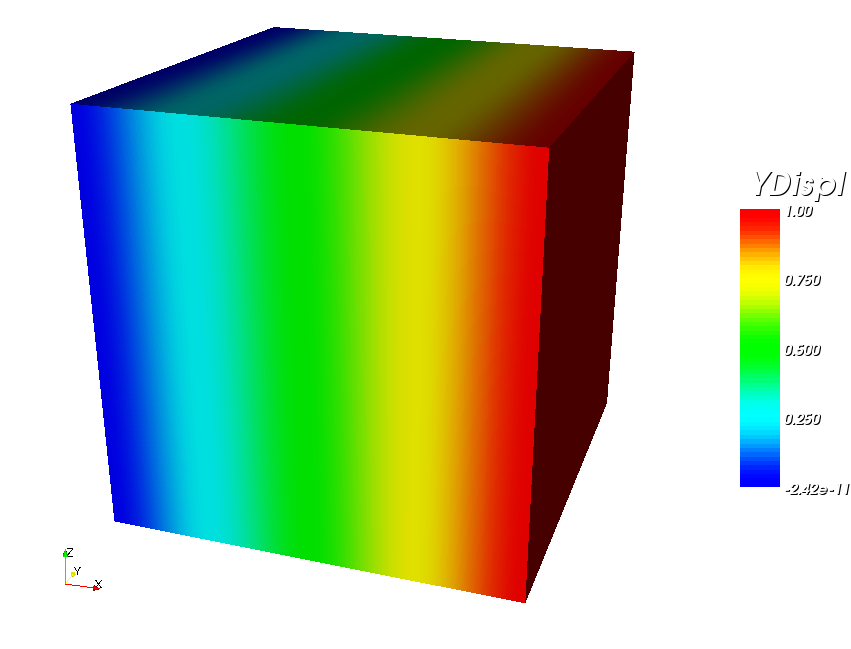
\includegraphics{figs/ydisp_t0.eps}
      \caption{ParaView rendering of displacement in y-direction at
        time step 0 (elastic solution to the imposed dislocation) for
        the simple strike-slip example.}
      \label{fig:splitcube:ydisp:t0}
    \end{center}
  \end{figure}
  
\item In the \guibutton{Display} tab, you can change several options,
  such as including a color bar, coloring a different component,
  interpolating colors, and changing the color map.
\item Let's show the displacements as vectors. Click on the calculator
  icon, and add the three displacement components together. Enter
  \begin{screen}
  XDispl*iHat + YDispl*jHat + ZDispl*kHat
  \end{screen}
  in the \guimenuitem{Calculator} box. Note the variable names are
  available by clicking on the \guibutton{scalars} button and the
  \guibutton{iHat}, \guibutton{jHat}, \guibutton{kHat} buttons are on
  the right side of the top row. Click on the \guibutton{Accept}
  button. To show the dataset as vectors, click on the
  \guibutton{glyph} button (looks like several dots) in the toolbar.
  After clicking the \guibutton{Accept} button, you should have a
  vector plot. You can turn on/off other datasets by clicking on the
  eye icon to the left of the dataset name. If you color the surfaces
  using the x-displacements field while also making the displacement
  vectors visible (colored using property), you should see an image
  similar to the one in figure~\ref{fig:splitcube:ydisp:vec:t0}.

  \begin{figure}[htbp]
    \begin{center}
      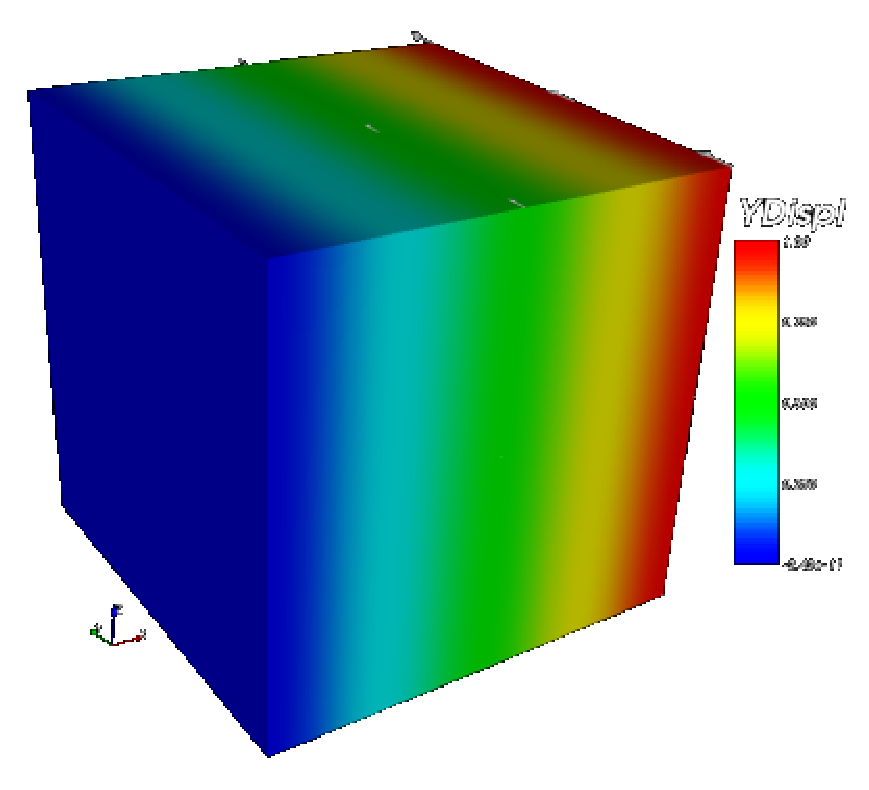
\includegraphics{figs/ydisp_vec_t0}
      \caption{ParaView rendering of displacement in y-direction and
        displacement vectors at time step 0 (elastic solution to the
        imposed dislocation) for the simple strike-slip example.}
      \label{fig:splitcube:ydisp:vec:t0}
    \end{center}
  \end{figure}      

\end{enumerate}

\subsection{Run the simulation on two processors}

In this step we will run the simulation on two processors. Even if
your machine only has one processor, a "multprocessor" job will run as
multiple processes on the single processor. In such cases, the job
will run slower than the single processor run, but the two processes
will behave independently as if they are on different processors.

\begin{enumerate}
\item Run \command{tutor.py} for step "run2" with mode "retrieve" to
  make sure all parameter files are available.

  \begin{screen}
    \shellprompt\userinput{./tutor.py -m retrieve -s run2}
  \end{screen}
  
\item The parameter files are the same as those in the single
  processor run. The \command{runbm.py} script will automatically take
  care of duplicating these files so that there is one for each
  processor.
\item Run the simulation by executing \command{runbm.py -n 2}, where
  the 2 refers to the number of processors.

  \begin{screen}
    \shellprompt\userinput{./runbm.py -n 2}
  \end{screen}
\end{enumerate}

\subsection{Visualize the two processor run}

PyLith does not currently support parallel output, so each processor
writes its UCD output to a different file. This means that you need to
form complete UCD files for each processor and then load each one into
\application{ParaView}.

\begin{enumerate}
\item If necessary, run \command{tutor.py} for step "viz2" with mode
  "retrieve" to fetch the simulation output from the archive.

  \begin{screen}
    \shellprompt\userinput{./tutor.py -m retrieve -s viz2}
  \end{screen}
  
\item As in the case of the single processor run, the first step is to
  combine the mesh topology information with the output at a given
  time step into a complete UCD file. Because PyLith writes the output
  from each processor into a different file, we must run \command{cat}
  twice to create UCD files for each processor.

  \begin{screen}
    \shellprompt\userinput{cat splitcube\_2.0.mesh.inp splitcube\_2.0.mesh.time.00000.inp \(\backslash\)}
      \userinput{> splitcube\_2.0.mesh.t00000.inp}
    \shellprompt\userinput{cat splitcube\_2.1.mesh.inp splitcube\_2.1.mesh.time.00000.inp \(\backslash\)}
      \userinput{> splitcube\_2.1.mesh.t00000.inp}
  \end{screen}

\item Start \application{ParaView} by executing \command{paraview}.

  \begin{screen}
    \shellprompt\userinput{paraview}
  \end{screen}
  
\item Load the UCD files that you just created by selecting
  \guimenu{File}\guiselect\guimenuitem{Open Data}. Select the file in
  the dialog box and the click the \guibutton{Open} button. Click the
  \guibutton{Accept} button. You can now visualize the datasets just
  like you did for the single processor case.
\item You can merge the datasets from the different processors by
  selecting \guimenu{Filter}\guiselect\guimenuitem{Append}. Doing so
  will allow you to operate on the data from all of the processors
  simultaneously instead of having to repeat any processing for every
  processor.
\end{enumerate}
